% Define the top matter
\renewcommand{\moduleTitle}{\textit{de novo} Assembly}
\renewcommand{\moduleAuthors}{%
  Matthias Haimel \mailto{mhaimel@ebi.ac.uk}\\
  Nathan S. Watson-Haigh \mailto{nathan.watson-haigh@awri.com.au}
} \renewcommand{\moduleContributions}{%
  
}

%  Start: Module Title Page
\chapterstyle{module}
\chapter{\moduleTitle}
\newpage
% End: Module Title Page

\section{Key Learning Outcomes}

TODO

\section{Resources You'll be Using}
Although we have provided you with an environment which contains all the tools
and data you will be using in this module, you may like to know where we have
sourced those tools and data from.
 
\subsection{Tools Used}
\begin{description}[style=multiline,labelindent=0cm,align=left,leftmargin=1cm]
  \item[Velvet] \hfill\\
  	\url{http://www.ebi.ac.uk/~zerbino/velvet/}
  \item[AMOS Hawkeye] \hfill\\
    \url{http://apps.sourceforge.net/mediawiki/amos/index.php?title=Hawkeye}
  \item[gnx-tools] \hfill\\
    \url{https://github.com/mh11/gnx-tools}
  \item[FastQC] \hfill\\
    \url{http://www.bioinformatics.bbsrc.ac.uk/projects/fastqc/}
\end{description}

\subsection{Sources of Data}
\begin{itemize}
\item \url{http://www.ebi.ac.uk/ena/data/view/SRS004748}
\item \url{ftp://ftp.sra.ebi.ac.uk/vol1/fastq/SRR022/SRR022825/SRR022825.fastq.gz}
\item \url{ftp://ftp.sra.ebi.ac.uk/vol1/fastq/SRR022/SRR022823/SRR022823.fastq.gz}
\item \url{http://www.ebi.ac.uk/ena/data/view/SRS004748}
\item \url{ftp://ftp.ensemblgenomes.org/pub/release-8/bacteria/fasta/Staphylococcus/s_aureus_mrsa252/dna/s_aureus_mrsa252.EB1_s_aureus_mrsa252.dna.chromosome.Chromosome.fa.gz}
\item \url{ftp://ftp.sra.ebi.ac.uk/vol1/fastq/SRR022/SRR022852/SRR022852_1.fastq.gz}
\item \url{ftp://ftp.sra.ebi.ac.uk/vol1/fastq/SRR022/SRR022852/SRR022852_2.fastq.gz}
\item \url{ftp://ftp.sra.ebi.ac.uk/vol1/fastq/SRR023/SRR023408/SRR023408_1.fastq.gz}
\item \url{ftp://ftp.sra.ebi.ac.uk/vol1/fastq/SRR023/SRR023408/SRR023408_2.fastq.gz}
\item \url{ftp://ftp.sra.ebi.ac.uk/vol1/fastq/SRR000/SRR000892/SRR000892.fastq.gz}
\item \url{ftp://ftp.sra.ebi.ac.uk/vol1/fastq/SRR000/SRR000893/SRR000893.fastq.gz}
\item \url{http://www.ebi.ac.uk/ena/data/view/SRX007709}
\item \url{http://www.ebi.ac.uk/ena/data/view/SRX000181}
\end{itemize}

\newpage

\section{Introduction}
Some general introduction

\section{Prepare the Environment}
\begin{information}
The first exercise should get you comfortable with the computer environment. I
am going to assume that either you have some minimal experience with command
line UNIX, or that the very short introduction I should have given you by now
was sufficient. Please ask if neither of the above is true. It is not as tricky
as it looks \ldots honest!
\end{information}

\begin{steps}
First make sure that you are in your home directory by typing:
\begin{lstlisting}
cd
\end{lstlisting}

and making absolutely sure you're there by typing:
\begin{lstlisting}
pwd
\end{lstlisting}

Now create sub-directories for this and the two other velvet practicals. All
these directories will be made as sub-directories of a directory for the whole
course called NGS. For this you can use the following commands:
\begin{lstlisting}
mkdir -p NGS/velvet/{part1,part2,part3}
\end{lstlisting}
\end{steps}

\begin{information}
The \texttt{-p} tells \texttt{mkdir} (make directory) to make any parent
directories if they don't exist. You could create the directories one-at-a-time
by doing:
\begin{lstlisting}
mkdir NGS
mkdir NGS/velvet
mkdir NGS/velvet/part1
mkdir NGS/velvet/part2
mkdir NGS/velvet/part3
\end{lstlisting}
\end{information}

\begin{steps}
After creating the directories, examine the structure and move into the
directory ready for the first velvet exercise by typing:
\begin{lstlisting}
ls -R NGS
cd NGS/velvet/part1
pwd
\end{lstlisting}

\end{steps}

\section{Downloading and Compiling Velvet}
\begin{note}
For the duration of this workshop, all the software you require has been set up
for you already. This might not be the case when you return to �real life�. Many
of the programs you will need, including velvet, are quite easy to set up, it
might be instructive to try a couple.
\end{note}

\begin{information}
Although you will be using the preinstalled version of velvet, it is useful to
know how to compile velvet as some of the parameters you might like to control
can only be set at compile time. You can find the latest version of velvet at:

\center{\url{http://www.ebi.ac.uk/~zerbino/velvet/}}

You could go to this URL and download the latest velvet version, or
equivalently, you could type the following, which will download, unpack,
inspect, compile and execute your locally compiled version of velvet:
\begin{lstlisting}
cd ~/NGS/velvet/part1
pwd
cp ~/NGS/Data/velvet_1.2.07.tgz ./
tar xzf ~/NGS/Data/velvet_1.2.07.tgz
ls -R
cd velvet_1.2.07
make velveth velvetg
./velveth
\end{lstlisting}
\end{information}

\begin{steps}
Take a look at the executables you have created. They will be displayed as green
by the command:
\begin{lstlisting}
ls --color=always
\end{lstlisting}
\end{steps}

\begin{notes}
The switch \texttt{--color}, offensively misspelled in American!, instructs that
files be coloured according to their type. This is often the default. Here we
are just being cautious. The \texttt{=always} is included as colouring is
usually suppressed in scripts. If you run this exercise using the script
provided, just \texttt{--color} would not be enough. \texttt{--color=always}
insists on file colouring even from a script.
\end{notes}

\begin{steps}
Have a look of the output the command produces and you will see that
\texttt{MAXKMERLENGTH=31} and \texttt{CATEGORIES=2} parameters were passed into
the compiler.

This indicates that the default compilation was set for De Bruijn graph k-mers of
maximum size 31 and to allow a maximum of just 2 read categories. You can
override these, and other, default configuration choices using command line
parameters. Assume, you want to run velvet with a k-mer length of 41 using 3
categories, velvet needs to be recompiled to enable this functionality by
typing:
\begin{lstlisting}
make clean
make velveth velvetg MAXKMERLENGTH=41 CATEGORIES=3;
./velveth
\end{lstlisting}
\end{steps}

\begin{questions}
Discuss with the persons next to you the following questions:

What are the consequences of the parameters you have given make for velvet?

Why does Velvet use k-mer 31 and 2 categories as default?

Should you get better results by using a longer k-mer length?

\end{questions}

\begin{steps}
velvet can also be used to process SOLID colour space data. To do this you need
a further make parameter. With the following command clean away your last
compilation and try the following parameters:
\begin{lstlisting}
make clean
make MAXKMERLENGTH=41 CATEGORIES=3 color
./velveth_de
\end{lstlisting}

\end{steps}

\begin{questions}
What effect would the following compil-time parameters have on velvet:\\
\texttt{OPENMP=Y}

\texttt{LONGSEQUENCES=Y}

\texttt{BIGASSEMBLY=Y}

\texttt{VBIGASSEMBLY=Y}

\texttt{SINGLE\_COV\_CAT=Y}

\end{questions}

\begin{notes}
For a further description of velvet compile and runtime parameters please see
the velvet Manual: \url{https://github.com/dzerbino/velvet/wiki/Manual}
\end{notes}

\newpage
\section{Assembling Single-end Reads}

\begin{notes}
The data you will examine is from Staphylococcus aureus USA300 which has a
genome of around 3MB . The reads are Illumina and are unpaired, also known as
single-end library. Even though you have carefully installed velvet in your own
workspace, we will use a pre-installed version.

The data needed for this section can be obtained from the Sequence Read Archive
(SRA). For the following example use the run data SRR022825 and SRR022823 from
the SRA Sample SRS004748. The SRA experiment could be viewed by setting your
browser to the URL:

\center{\url{http://www.ebi.ac.uk/ena/data/view/SRS004748}}

\begin{warning}
We have already downloaded the data files for you.
\end{lstlisting}

\end{warning}
\end{notes}

\begin{information}
The following exercise focuses on velvet using single-end reads, how the
available parameters effect an assembly and how to measure and compare the
changes.
\end{information}

\begin{steps}
To begin with, first move back to the directory you prepared for this exercise,
create a new folder with a suitable name for this part and move into it. There
is no need to download1 the read files, as they are already stored locally.
Instead we will create soft links to the files. Continue by copying (or typing):
\begin{lstlisting}
cd ~/NGS/velvet/part1
mkdir SRS004748
cd SRS004748
pwd
ln -s ~/NGS/Data/SRR022825.fastq.gz ./
ln -s ~/NGS/Data/SRR022823.fastq.gz ./
ls -l
\end{lstlisting}
\end{steps}

\begin{information}
You are ready to process your data with velvet, which is a compressed fastq file.
Velvet has two main components:
\begin{description}[style=multiline,labelindent=1cm,align=left,leftmargin=2cm]
  \item[velveth] \hfill\\
    Used to construct, from raw read data, a dataset organised in the
    fashion expected by the   second component, velvetg.
  \item[velvetg] \hfill\\
    The core of velvet where the de Bruijn graph assembly is built and
    manipulated.
\end{description}

You can always get further information about the usage of both velvet programs
by typing \texttt{velvetg} or \texttt{velveth} in your terminal.
\end{information}

\begin{steps}
Now run velveth for the reads in \texttt{SRR022825.fastq.gz} and
\texttt{SRR022823.fastq.gz} using the following options:
\begin{itemize}
  \item A de Bruijn graph k-mer of 25
  \item An output directory called run\_25
\end{itemize}
\begin{lstlisting}
velveth run_25 25 -fastq.gz -short SRR022825.fastq.gz SRR022823.fastq.gz
\end{lstlisting}

\texttt{velveth} talks to itself for a while and ends with some files in the
output directory. Move into the output directory \texttt{run\_25} and take a look
around at what \texttt{velveth} had done so far. The UNIX command \texttt{less}
allows you to look at output files (press \texttt{q} for quit). Just in case you
still need a hint:

\begin{lstlisting}
cd run_25
ls -l
head Sequences
cat Log
\end{lstlisting}

\end{steps}

\begin{questions}
What did you find in the folder \texttt{run\_25}?

\vspace{2cm}

Describe the content of the two \texttt{velveth} output files?

\vspace{2cm}

What does the \texttt{Log} file store for you?

\vspace{2cm}
\end{questions}

\begin{steps}
Now move one directory level up and run velvetg on your output directory, with
the commands:
\begin{lstlisting}
cd ../
time velvetg run_25
\end{lstlisting}

Move back into your results directory to examine the effects of velvetg:
\begin{lstlisting}
cd run_22
ls -l
\end{lstlisting}

\begin{questions}
What extra files do you see in the folder \texttt{run\_25}?

\vspace{2cm}

What do you suppose they might represent?

\vspace{2cm}
  
In the Log file in \texttt{run\_25}, what is the N50?

\vspace{2cm}

\end{questions}

\begin{information}
Hopefully, we will have discussed what the N50 statistic is by this point.
Broadly, it is the median (not average) of a sorted data set using the length of
a set of sequences. Usually it is the length of the contig whose length, when
added to the length of all longer contigs, makes a total greater that half the
sum of the lengths of all contigs. Easy, but messy � a more formal definition
can be found here:

\center{\url{http://www.broadinstitute.org/crd/wiki/index.php/N50}}
\end{information}

\begin{steps}
Backup the \texttt{contigs.fa} file and calculate the N50 (and the N25,N75) value with
the command:
\begin{lstlisting}
cp contigs.fa contigs.fa.0
gnx -min 100 -nx 25,50,75 contigs.fa
\end{lstlisting}

\end{steps}

\begin{questions}
Does the value of N50 agree with the value stored in the Log file?

\vspace{2cm}

If not, why do you think this might be?

\vspace{2cm}

\end{questions}

\begin{information}
In order to improve our results, take a closer look at the standard options of
\texttt{velvetg} by typing \texttt{velvetg} without parameters. For the moment
focus on the two options \texttt{-cov\_cutoff} and \texttt{-exp\_cov}. Clearly
\texttt{-cov\_cutoff} will allow you to exclude contigs for which the k-mer
coverage is low, implying unacceptably poor quality.
The \texttt{-exp\_cov} switch is used to give \texttt{velvetg} an idea of the
coverage to expect.

If the expected coverage of any contig is substantially in excess of the
suggested expected value, maybe this would indicate a repeat. For further
details of how to choose the parameters, go to 'Choice of a coverage cutoff':

\center{\url{http://wiki.github.com/dzerbino/velvet/}}

\end{information}

\begin{steps}
Briefly, the k-mer coverage (and much more information) for each contig is stored
in the file \texttt{stats.txt} and can be used with R to visualize the coverage
distribution. Take a look at the \texttt{stats.txt} file, start R, load and
visualize the data using the following commands:
\begin{lstlisting}
R --no-save --no-restore
library(plotrix)
data <- read.table("stats.txt", header=TRUE)
weighted.hist(data$short1_cov, data$lgth, breaks=0:50)
\end{lstlisting}

A weighted histogram is a better way of visualizing the coverage information,
because of noise (lots of very short contigs). You can see an example output
below:

\begin{figure}[H]
\centering
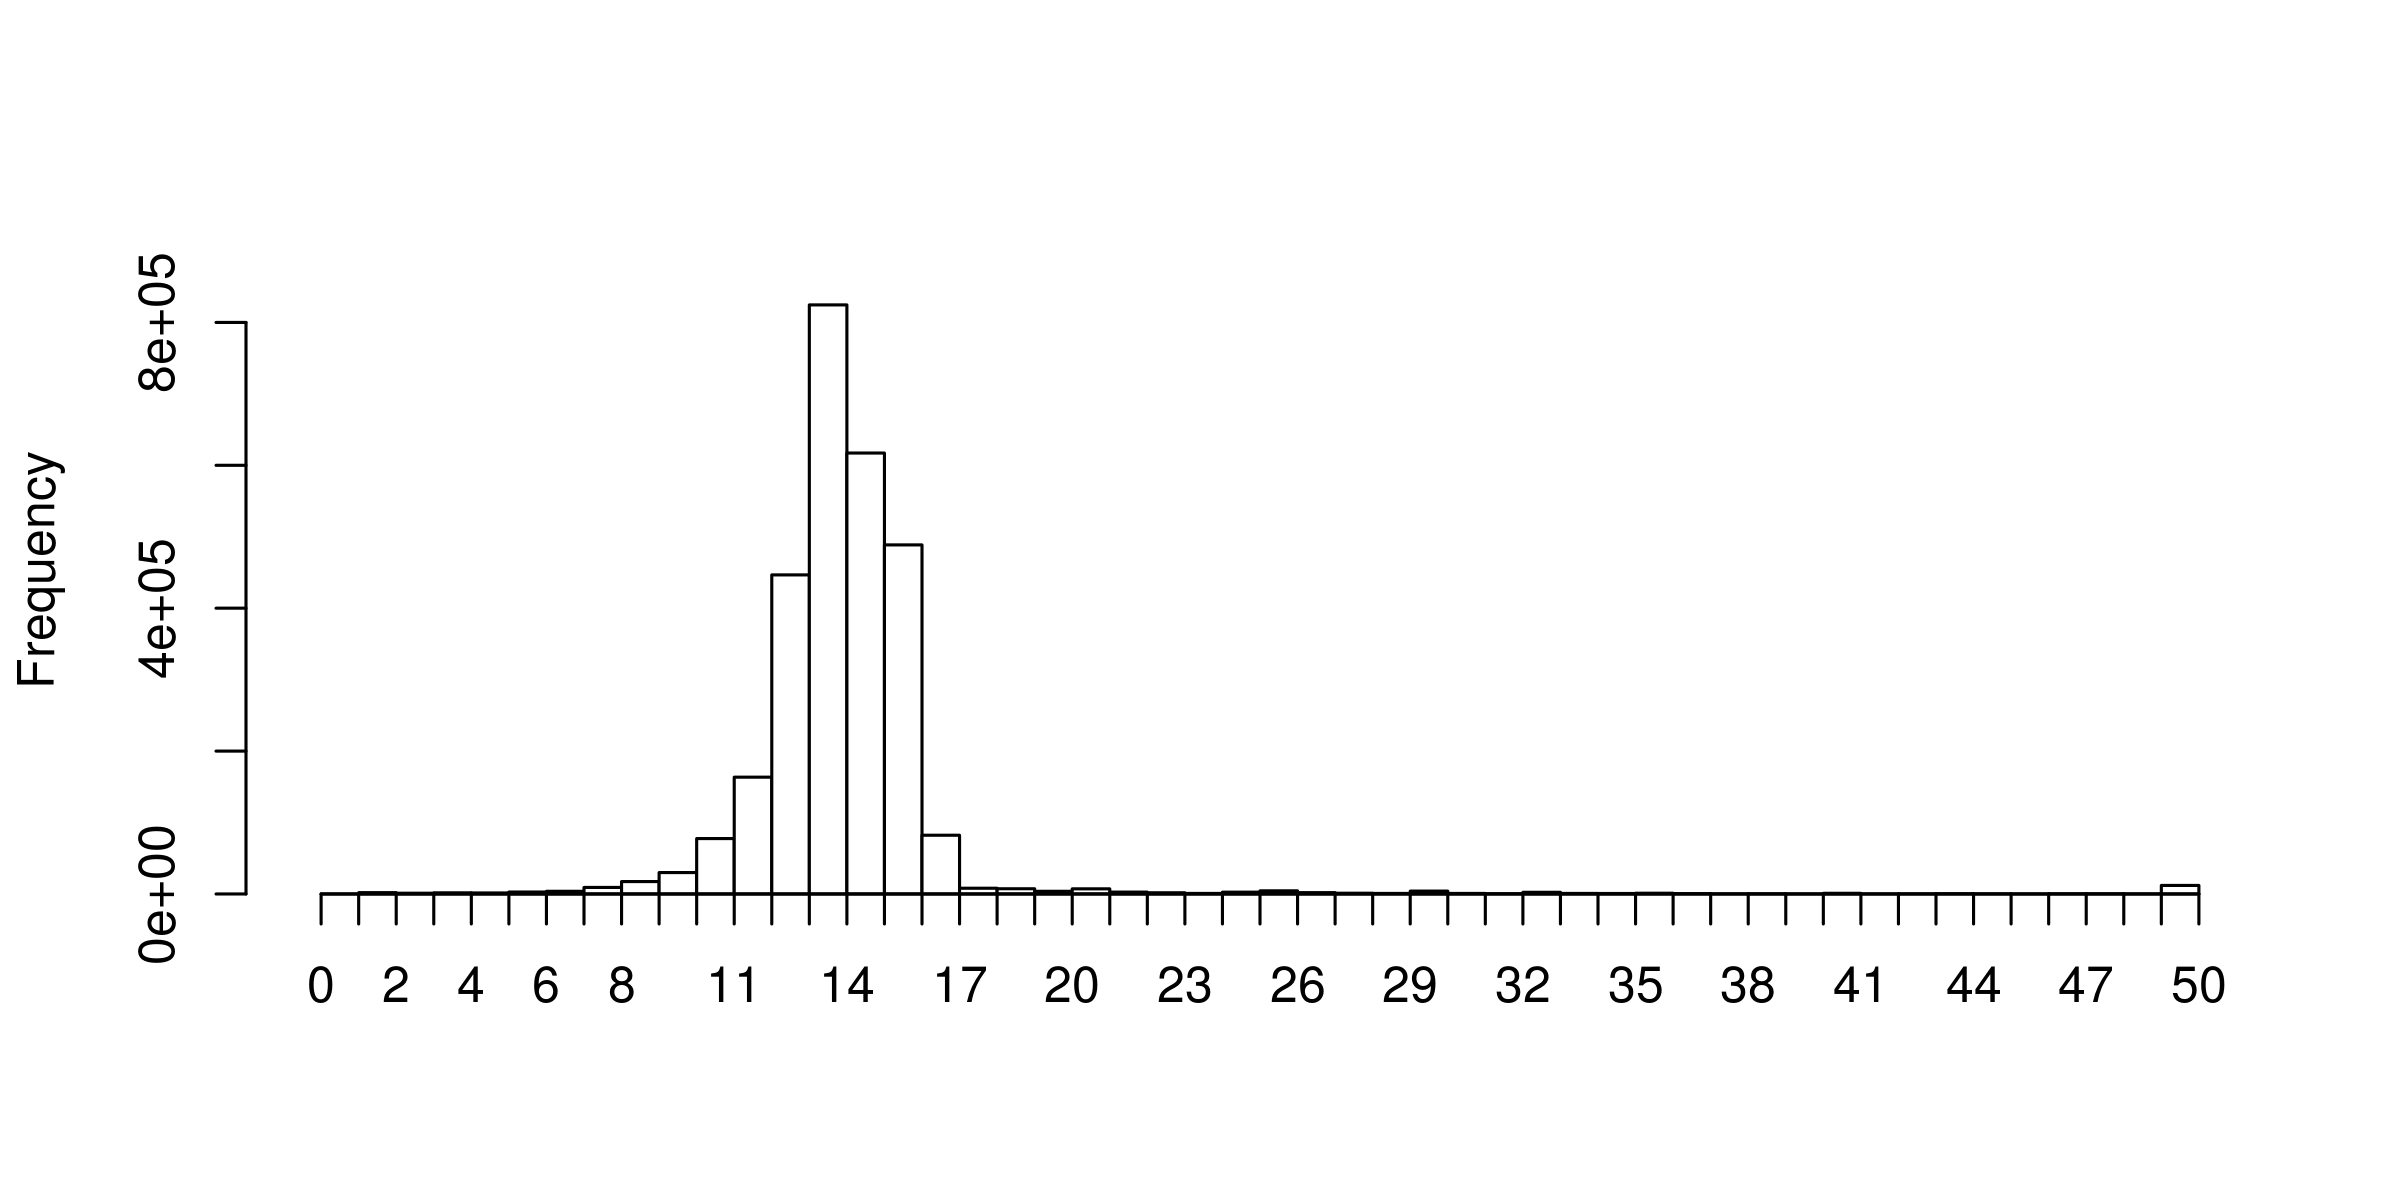
\includegraphics[width=0.8\textwidth]{de_novo/velvet_Rplot001.png}
\label{fig:SRS004748_coverage_hist}
\end{figure}

After choosing the expected coverage and the coverage cut-off, you can exit R by
typing:
\begin{lstlisting}
q()
\end{lstlisting}
\end{steps}

\begin{steps}
The weighted histogram suggests to me that the expected coverage is around 14
and that everything below 6 is likely to be noise. Some coverage is also
represented at around 20, 30 and greater 50, which might be contamination or
repeats (depending on the dataset), but at the moment this should not worry you.
To see the improvements, rerun velvetg first with \texttt{-cov\_cutoff} 6 and
after checking the N50 use only / add \texttt{-exp\_cov} 14 to the command line
option. Also keep a copy of the contigs file for comparison:
\begin{lstlisting}
cd ~/NGS/velvet/part1/SRS004748
time velvetg run_25 -cov_cutoff 6

# Make a copy of the run
cp run_25/contigs.fa run_25/contigs.fa.1

time velvetg run_25 -exp_cov 14
cp run_25/contigs.fa run_25/contigs.fa.2

time velvetg run_25 -cov_cutoff 6 -exp_cov 14
cp run_25/contigs.fa run_25/contigs.fa.3
\end{lstlisting}
\end{steps}

\begin{questions}
What is the N50 with no parameter:

What is the N50 with \texttt{-cov\_cutoff} 6:

What is the N50 with \texttt{-exp\_cov} 14:

What is the N50 with \texttt{-cov\_cutoff} 6 \texttt{-exp\_cov} 14:

Did you notice a variation in the time velvetg took to run? If so, can you
explain why that might be?

\end{questions}

\begin{steps}
You were running \texttt{velvetg} with the \texttt{-exp\_cov} and
\texttt{-cov\_cutoff} parameters. Now try to experiment using different
cut-offs, expected parameters and also explore other settings (e.g.
\texttt{-max\_coverage}, \texttt{-max\_branch\_length}, \texttt{-unused\_reads},
\texttt{-amos\_file}, \texttt{-read\_trkg} or see \texttt{velvetg} help menu).
\end{steps}

\begin{questions}
Make some notes about the parameters you've played with and the results you
obtained. Please also comment on the \texttt{-max\_coverage} and
\texttt{-max\_branch\_length} parameters.

\vspace{4\questionspacing}

\end{questions}


\begin{note}
In particular, look at the \texttt{-amos\_file} parameter which instructs
\texttt{velvetg} to create a version of the assembly that can be processed and
viewed with a program called AMOS Hawkeye. Another program, called tablet, can
also understand and display the AMOS file. For now, we will take a look at
Hawkeye.
\end{note}

\begin{steps}
Run velvetg with just \texttt{-cov\_cutoff} 6 but requesting an amos file:
\begin{lstlisting}
velvetg run_25 -cov_cutoff 6 -amos_file yes
\end{lstlisting}

Now convert the AMOS message file \texttt{velvet\_asm.afg} into an AMOS bank and
view the assembly using AMOS Hawkeye.
\begin{lstlisting}
bank-transact -c -b run_25/velvet_asm.bnk -m run_25/velvet_asm.afg
hawkeye run_25/velvet_asm.bnk
\end{lstlisting}

Once the file has loaded in Hawkeye, select and display one of the longer
contigs. Select the Contigs tab on the top of Hawkeye and take a closer look at
the Contigs information. Note the lack of Read information and the one
dimensional nature of the Contigs display. Close down Hawkeye when you have seen
enough and delete the AMOS bank file.
\begin{lstlisting}
rm -r run_25/velvet_asm.bnk
\end{lstlisting}

\end{steps}

\begin{steps}
Now rerun velvetg adding the additional parameter \texttt{-exp\_cov} 14 with no
need to save any files as the AMOS file needs to be changed.
\begin{lstlisting}
velvetg run_25 -cov_cutoff 6 -exp_cov 14 -amos_file yes
\end{lstlisting}

Again, convert the AMOS message file into an AMOS bank and view the assembly
using Hawkeye or tablet:
\begin{lstlisting}
bank-transact -c -b run_25/velvet_asm.bnk -m run_25/velvet_asm.afg
hawkeye run_25/velvet_asm.bnk
\end{lstlisting}

\begin{figure}[H]
\centering
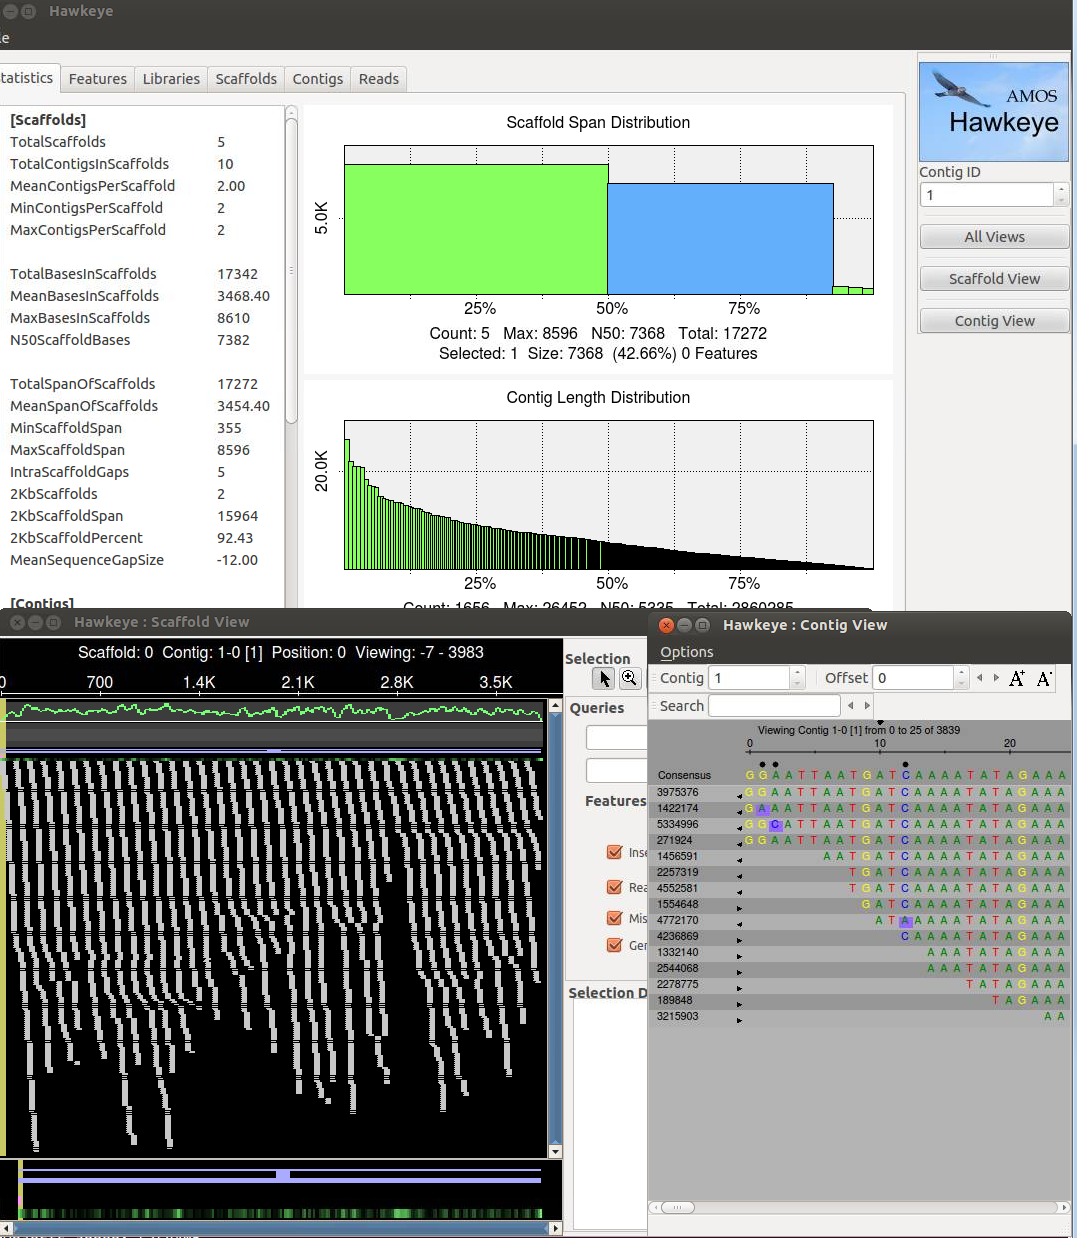
\includegraphics[width=0.8\textwidth]{de_novo/hawkeye_single_ended.png}
\caption{You should get a similar looking result with Hawkeye. If you are happy that you explored enough functionality, close down Hawkeye and continue with the exercise.}
\label{fig:hawkeye_single_ended}
\end{figure}

\end{steps}

\begin{questions}
Why do you think there was read information only for the second use of Hawkeye
and tablet?
  
You may have noticed velvetg took a little longer with \texttt{-exp\_cov} 14 on.
Does this make sense?

\end{questions}


\begin{bonus}
If you want to explore the behaviour of velvet even further, you could
experiment with the following.

Reduce the sequence coverage by only choosing one input file for the assembly
e.g. \texttt{SRR022825.fastq.gz}

Increase the sequence coverage by downloading further files from the same ENA
sample SRS004748 \url{http://www.ebi.ac.uk/ena/data/view/SRS004748}.

\begin{questions}
How did the N50 change by a) reducing the coverage and b) increasing the coverage:

\vspace{4\questionspacing}

\end{questions}

\end{bonus}

\subsection{Simple Assembly Simulation}

\begin{notes}
The data for this section is from Staphylococcus aureus MRSA252, a genome
closely related to the genome that provided the short read data in the earlier
sections of this exercise. The sequence data this time is the fully assembled
genome. The genome size is therefore known exactly and is 2,902,619 bp.
\end{notes}

\begin{information}
In this exercise you will process the single whole genome sequence with velveth
and velvetg, look at the output only and go no further. The main intent of
processing this whole genome is to compute its N50 value. This must clearly be
very close to the ideal N50 value for the short reads assembly and so aid
evaluation of that assembly.
\end{information}

\begin{steps}
To begin, move back to the main directory for this exercise, make a
sub-directory for the processing of this data and move into it. All in one go,
this would be:
\begin{lstlisting}
cd ~/NGS/velvet/part1/ 
mkdir MRSA252 
cd MRSA252
\end{lstlisting}

Next, you need to download the genome sequence from
\url{http://www.ensemblgenomes.org/} which holds five new sites, for bacteria,
protists, fungi, plants and invertebrate metazoa. You could browse for the data
you require or use the file which we have downloaded for you. For the easier of
these options, make and check a soft link to the local file and with the
commands:
\begin{lstlisting}
ln -s ~/NGS/Data/s_aureus_mrsa252.EB1_s_aureus_mrsa252.dna.chromosome.Chromosome.fa.gz ./
ls -l
\end{lstlisting}

\end{steps}

\begin{notes}
Usually Velvet expects relatively short sequence entries and for this reason has
a read limit of 32,767 bp per sequence entry. As the genome size is 2,902,619 bp
- longer as the allowed limit and does not fit with the standard settings into
velvet. But like the maximum k-mer size option, you can tell Velvet during
compile time, using \texttt{LONGSEQUENCES=Y}, to expect longer input sequences
than usual. I already prepared the executable which you can use by typing
\texttt{velveth\_long} and \texttt{velvetg\_long}.
\end{notes}

\begin{steps}
Now, run \texttt{velveth\_long}, using the file you either just downloaded or created a
soft link to as the input:
\begin{lstlisting}
velveth_long run_25 25 -fasta.gz -long s_aureus_mrsa252.EB1_s_aureus_mrsa252.dna.chromosome.Chromosome.fa.gz
velvetg_long run_25
\end{lstlisting}

\end{steps}

\begin{questions}
What is the N50?

How does the N50 compare to the previous single end run (SRS004748)?
  
Does the total length differ from the input sequence length?
  
What happens when you rerun velvet with a different k-mer length?

\end{questions}



\section{Assembling Paired-end Reads}

\begin{note}
The data you will examine in this exercise is again from Staphylococcus aureus
which has a genome of around 3MB. The reads are Illumina paired end with an
insert size of 350 bp.

The required data can be downloaded from the SRA. Specifically, the run data
(SRR022852) from the SRA Sample SRS004748.

\center{\url{http://www.ebi.ac.uk/ena/data/view/SRS004748}}

\end{note}

\begin{information}
The following exercise focuses on preparing the paired-end FASTQ files ready for
velvet, using velvet in paired-end mode and comparing results with velvet's
'auto' option.
\end{information}

\begin{steps}
First move to the directory you made for this exercise and make a suitable named
directory for the exercise:
\begin{lstlisting}
cd ~/NGS/velvet/part2 
mkdir SRS004748 
cd SRS004748
\end{lstlisting}

There is no need to download1 the read files, as they are already stored
locally. You will simply create a soft link to this pre-downloaded data using
the following commands:
\begin{lstlisting}
ln -s ~/NGS/Data/SRR022852_?.fastq.gz ./
\end{lstlisting}

It would be interesting to monitor the way that the programs you will run
utilize your computer's resources, particularly memory. A simple way to do this
is to open a second terminal and in it type:
\begin{lstlisting}
top
\end{lstlisting}
\end{steps}

\begin{note}
\texttt{top} is a program that continually monitors all the processes running on
your computer, showing the resources used by each. Alternatively you could use a
system monitor from your operating system as well. Leave this running and refer
to it at intervals, especially when programs appear to be taking a long time, of
just whenever your curiosity gets the better of you. You should find that as
this practical progresses, memory usage will increase significantly, but
hopefully not beyond the capacity of your workstation.

Now, back to the first terminal, you are ready to run \texttt{velveth} and \texttt{velvetg}. The
reads are \texttt{-shortPaired} this time and for the first run you should not use any
parameters for \texttt{velvetg}.
\end{note}

\begin{information}
From this point on, where it will be informative, time
your runs. This is very easy to do, just prefix the command to run the program
with the command \texttt{time}. This will cause UNIX to report how long the program took
to complete its task.
\end{information}

\begin{steps}
Set the two stages of velvet running, whilst you watch the memory usage as
reported by \texttt{top}. time the \texttt{velvetg} stage. The commands to enter
are:
\begin{lstlisting}
velveth run_25 25 -fmtAuto -create_binary -shortPaired -separate SRR022852_1.fastq.gz SRR022852_2.fastq.gz
time velvetg run_25
\end{lstlisting}

\end{steps}

\begin{questions}
Have you found what \texttt{-fmtAuto} and \texttt{-create\_binary} do? (see help menu)

Comment on the use of memory and CPU for \texttt{velveth} and \texttt{velvetg}?
 
How long did \texttt{velvetg} take?

\end{questions}

\begin{steps}
Next, after saving your \texttt{contigs.fa} file from being overwritten, set the
cut-off parameters that you investigated in the previous exercise and rerun
\texttt{velvetg}.
time and monitor the use of resources as previously. Start with
\texttt{-cov\_cutoff 16} thus:
\begin{lstlisting}
mv run_25/contigs.fa run_25/contigs.fa.0
time velvetg run_25 -cov_cutoff 16
\end{lstlisting}

Up until now, \texttt{velvetg} has ignored the paired-end information. Now try
running
\texttt{velvetg} with both \texttt{-cov\_cutoff 16} and \texttt{-exp\_cov 26}, but first save your \texttt{contigs.fa}
file. By using \texttt{-cov\_cutoff} and \texttt{-exp\_cov}, \texttt{velvetg}
tries to estimate the insert length, which you will see in the \texttt{velvetg}
output. The command is, of course:
\begin{lstlisting}
mv run_25/contigs.fa run_25/contigs.fa.1
time velvetg run_25 -cov_cutoff 16 -exp_cov 26
\end{lstlisting}

\end{steps}

\begin{questions}
Comment on the time required, use of memory and CPU for \texttt{velvetg}?
  
Which insert length does Velvet estimate?

\end{questions}

\begin{steps}
Next try running \texttt{velvetg} in `paired-end mode`. This entails running \texttt{velvetg}
specifying the insert length with the parameter \texttt{-ins\_length} set to 350. Even
though velvet estimates the insert length it is always advisable to check /
provide the insert length manually as velvet can get the statistics wrong due
to noise. Just in case, save your last version of \texttt{contigs.fa}. The commands are:
\begin{lstlisting}
mv run_25/contigs.fa run_25/contigs.fa.2
time velvetg run_25 -cov_cutoff 16 -exp_cov 26 -ins_length 350
mv run_25/contigs.fa run_25/contigs.fa.3
\end{lstlisting}
\end{steps}

\begin{questions}
How fast was this run?

\end{questions}

\begin{steps}
Take a look into the Log file.
\end{steps}

\begin{questions}
What is the N50 value for the \texttt{velvetg} runs using the switches:\\
\texttt{-cov\_cutoff 16}

\texttt{-cov\_cutoff 16 -exp\_cov 26}

\texttt{-cov\_cutoff 16 -exp\_cov 26 -ins\_length 350}

\end{questions}

\begin{steps}
Try giving the \texttt{-cov\_cutoff} and/or \texttt{-exp\_cov} parameters the
value \texttt{auto} - the \texttt{velvetg} help output could show you how. The
information Velvet prints during running includes information about the values
used (coverage cut-off or insert length) when using the \texttt{auto} option.
\end{steps}

\begin{questions}
Which coverage values does Velvet choose (hint: look at the output which velvet
produces while running)?

How does the N50 value change?
\end{questions}

\begin{steps}
Run \texttt{gnx} on all the \texttt{contig.fa} files you have generated in the
course of this exercise. The command will be:
\begin{lstlisting}
gnx -min 100 -nx 25,50,75 run_25/contigs.fa*
\end{lstlisting}
\end{steps}

\begin{questions}
For which runs are there Ns in the \texttt{contigs.fa} file and why? 
  
Comment on the number of contigs and total length generated for each run.
\end{questions}


\begin{bonus}
Similar to the single-end assembly you created previously, we can output a
paired-end assembly as an AMOS message format file. This file can then be
converted into an AMOS bank and viewed using AMOS Hawkeye.
\begin{lstlisting}
time velvetg run_25 -cov_cutoff 16 -exp_cov 26 -ins_length 350 -amos_file yes -read_trkg yes 
time bank-transact -c -b run_25/velvet_asm.bnk -m run_25/velvet_asm.afg         
hawkeye run_25/velvet_asm.bnk
\end{lstlisting}

\begin{questions}
Looking at the scaffold view of a contig, comment on the proportion of happy
mates to compressed mates.

What is the mean and standard deviation of the insert size report in the
Libraries tab of Hawkeye?

Look at the actual distribution of insert sizes for this library. Can you
explain where there is a difference between the mean and SD reported in those
two places?
\end{questions}

\begin{steps}
You can get AMOS to re-estimate the mean and SD of insert sizes. First, close
Hawkeye and then run the following commands before reopening the AMOS bank to
see what has changed.
\begin{lstlisting}
asmQC -b run_25/velvet_asm.bnk -scaff -recompute -update -numsd 2
hawkeye run_25/velvet_asm.bnk
\end{lstlisting}
\end{steps}

\begin{questions}
Looking at the scaffold view of a contig, comment on the proportion of happy
mates to compressed mates.

What is the mean and standard deviation of the insert size report in the
Libraries tab of Hawkeye?

Look at the actual distribution of insert sizes for this library. Does the mean
and SD reported in each of those two places now match?
\end{questions}
\end{bonus}

\subsection{Data Quality}
\begin{note}
As discussed previously, fastq format files include quality assessment of each
called base. As also mentioned earlier, velvet does not use this information
directly. However, by taking into account the quality of the read data, it
should be possible to both improve the efficiency (in terms of memory usage and
runtime) and the quality of the output.
\end{note}

\begin{information}
To investigate the effect of data quality, we will use the run data (SRR023408)
from the SRA experiment SRX008042. The reads are Illumina paired end with an
insert size of 92 bp.
\end{information}

\begin{steps}
As ever, move up a directory to the main directory for the whole of this
exercise and create and enter a new directory dedicated to this phase of the
exercise. The commands are:
\begin{lstlisting}
cd ~/NGS/velvet/part2 
mkdir SRX008042 
cd SRX008042
\end{lstlisting}

Create soft links to the read data files we downloaded for you from the SRA with
the command:
\begin{lstlisting}
ln -s ~/NGS/Data/SRR023408_?.fastq.gz ./
\end{lstlisting}
\end{steps}

\begin{note}
To look at the quality scores, you could use a tool called FastQC to process and
present the scores in a compact manner of basic statistics. FastQC can be
downloaded from:

\center{\url{http://www.bioinformatics.bbsrc.ac.uk/projects/fastqc/}}

Where there are links to an excellent manual and an even more excellent youtube
video. I hope to show you the video and recommend you keep the manual pages open
whilst you are using FastQC in this exercise.
\end{note}

\begin{steps}
Start up FastQC Graphical User Interface (GUI) to examine your compressed fastq
files by typing:
\begin{lstlisting}
fastqc &
\end{lstlisting}
\end{steps}

\begin{note}
The & sets FastQC running as a background job, thus freeing your terminal for
further commands if required. FastQC emerges as a big blank window.
\end{note}

\begin{steps}
Open both your compressed fastq files as was done in the video (Choose Open from
the File pull down menu, browse to your files, select them both and click OK).
Look at tabs for both files:
\end{steps}

\begin{figure}[H]
\centering
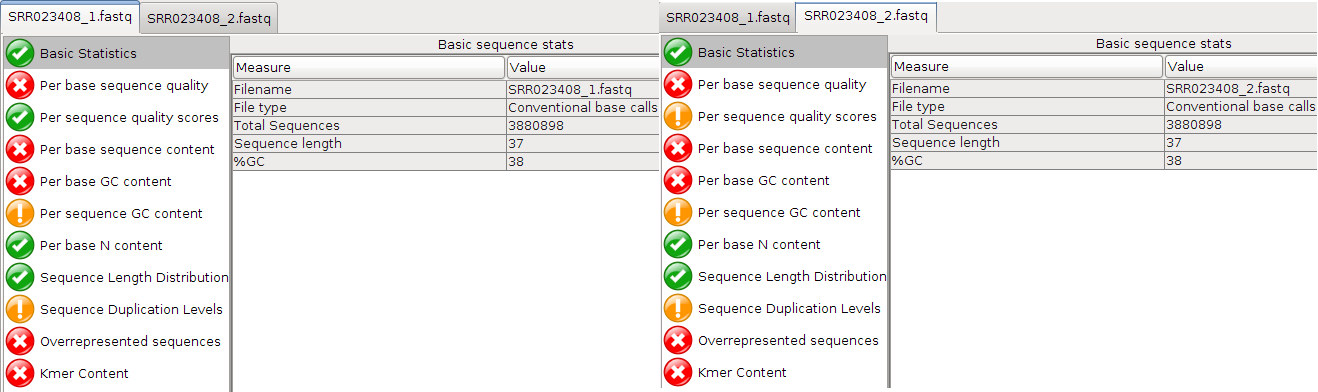
\includegraphics[width=0.8\textwidth]{de_novo/paired_fastqc.png}
\label{fig:paired_fastqc}
\end{figure}

\begin{questions}
Are the quality scores the same for both files?

Which value varies?

Take a look at the Per base sequence quality for both files. Did you note that it is not good for either file?

At which positions would you cut the reads off?

Why does the quality deteriorate towards the end of the read?

Does it make sense to trim the start?
\end{questions}

\begin{steps}
Have a look at the other options that fastqc offers. Make good use of the Help
to remind you of what you learned from the video. I suggest you open the Help
window and keep it on your screen, open at the relevant page, as you browse
through the fastqc possibilities.
\end{steps}

\begin{questions}
Which other statistics could you use to support your trimming strategy?
\end{questions}

\begin{figure}[H]
\centering
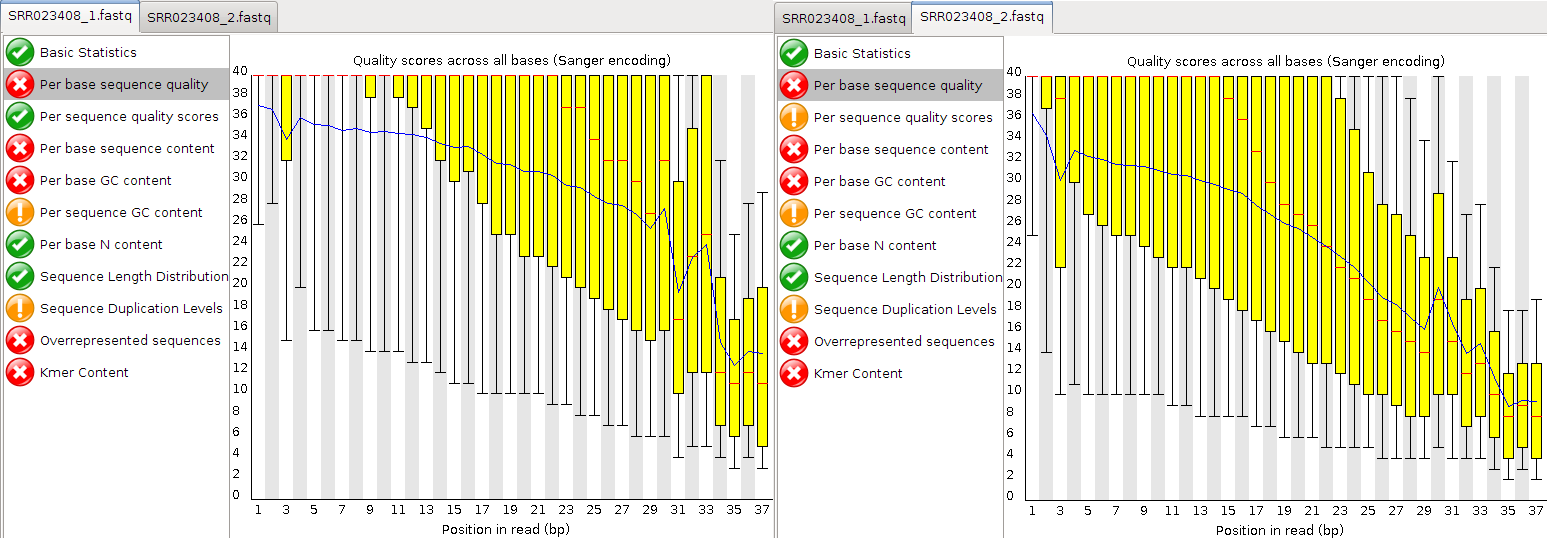
\includegraphics[width=0.8\textwidth]{de_novo/paired_fastqc_quality_plots.png}
\label{fig:paired_fastqc_quality_plots}
\end{figure}

\begin{steps}
Once you have decided how it might be sensible to trim your reads, close down
fastqc by selecting Exit from the File pull down menu. Now apply the knife to
your reads with \texttt{fastx\_trimmer} from the FASTX-Toolkit. However, you will
first need to decompress the FASTQ files. The usage of the tool can be found
here:

\url{http://hannonlab.cshl.edu/fastx_toolkit/commandline.html#fastx_trimmer_usage}

The suggestion (hopefully not far from your own thoughts?) is that you trim your
reads as follows:

\begin{lstlisting}
gunzip < SRR023408_1.fastq.gz > SRR023408_1.fastq
gunzip < SRR023408_2.fastq.gz > SRR023408_2.fastq
fastx_trimmer -Q 33 -f 4 -l 32 -i SRR023408_1.fastq -o SRR023408_trim1.fastq 
fastx_trimmer -Q 33 -f 3 -l 29 -i SRR023408_2.fastq -o SRR023408_trim2.fastq
\end{lstlisting}

Now run velveth with a k-mer value of 21 for both the untrimmed and trimmed read
files in \texttt{-shortPaired} mode. Separate the output of the two executions
of \texttt{velveth} into suitably named directories, followed by
\texttt{velvetg}. The commands would be:
\begin{lstlisting}
velveth run_21 21 -fmtAuto -create_binary -shortPaired -separate SRR023408_1.fastq SRR023408_2.fastq
time velvetg run_21

velveth run_21trim 21 -fmtAuto -create_binary -shortPaired -separate SRR023408_trim1.fastq SRR023408_trim2.fastq
time velvetg run_21trim
\end{lstlisting}
\end{steps}

\begin{questions}
What are the times for the two \texttt{velvetg} runs?

What N50 scores did you achieve?

What were the overall effects of trimming?
\end{questions}

\begin{steps}
The evidence is that trimming improved the assembly. The thing to do surely, is
to run velvetg with the \texttt{-cov\_cutoff} and \texttt{-exp\_cov}. In order
to use \texttt{-cov\_cutoff} and \texttt{-exp\_cov} sensibly, you need to
investigate with R, as you did in the previous exercise, what parameter values
to use. To start up R and produce the weighted histograms, type:
\begin{lstlisting}
R --no-save
library(plotrix) 
data <- read.table("run_21/stats.txt", header=TRUE) 
data2 <- read.table("run_21trim/stats.txt", header=TRUE) 
x11()
par(mfrow=c(1,2))
weighted.hist(data$short1_cov, data$lgth, breaks=0:50)
weighted.hist(data2$short1_cov, data2$lgth, breaks=0:50)
\end{lstlisting}

\begin{figure}[H]
\centering
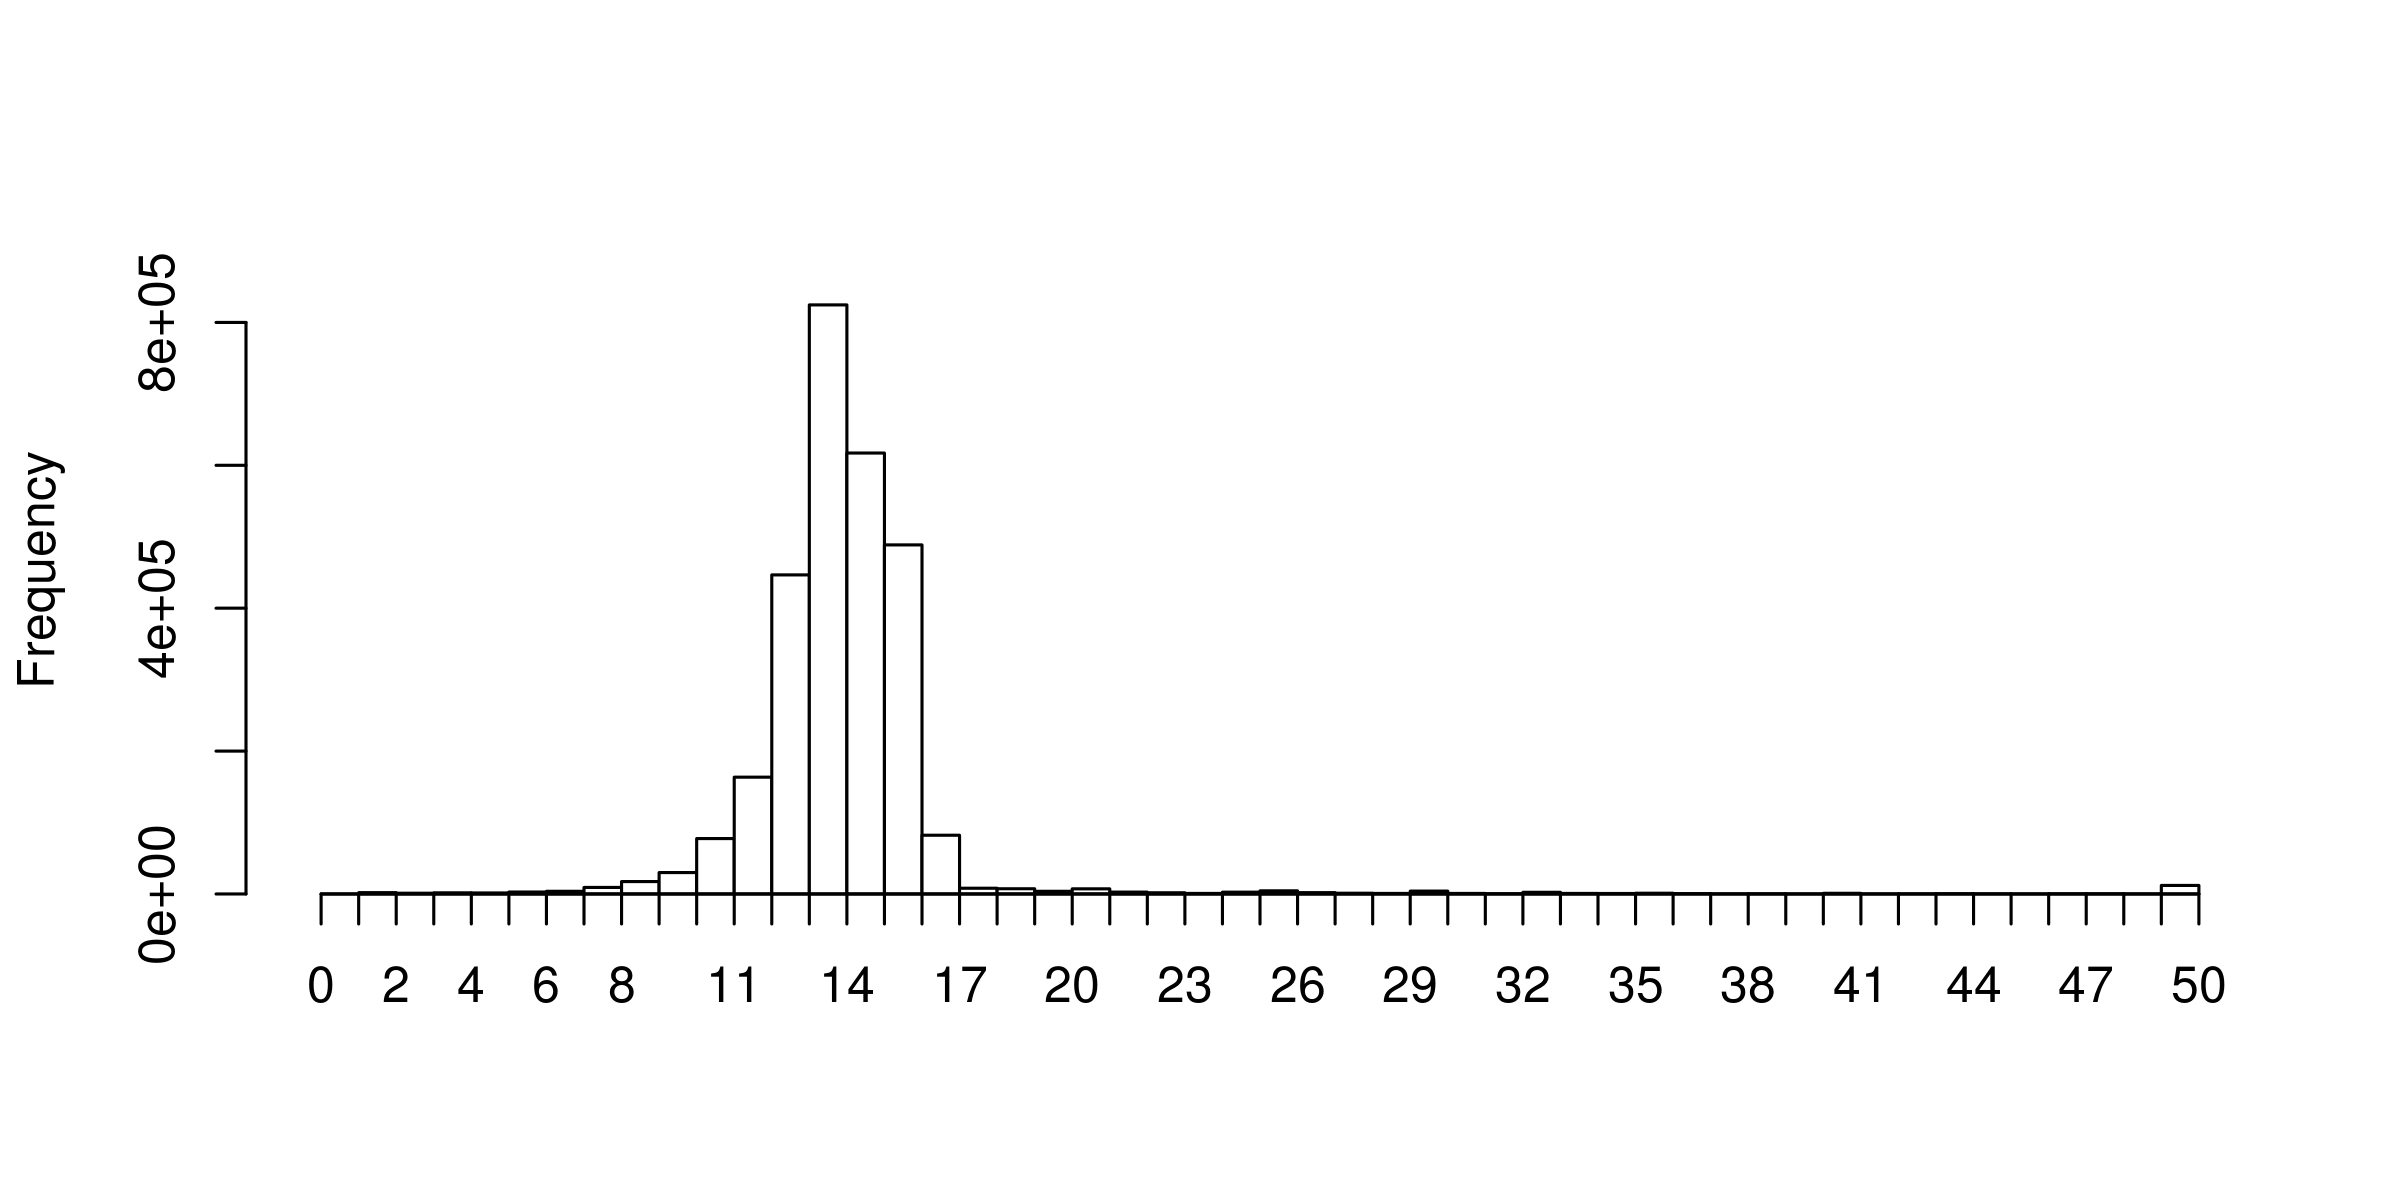
\includegraphics[width=0.8\textwidth]{de_novo/velvet_Rplot001.png}
\label{fig:velvet_Rplot001}
\end{figure}

One histogram suggests to me an expected coverage of around 13 with a coverage
cut-off of around 7. The trimmed histogram instead suggests an expected coverage
of around 9 with a coverage cut-off of around 5. If you disagree, feel free to
try different settings, but first leave R before running velvetg:
\begin{lstlisting}
q()

time velvetg run_21 -cov_cutoff 7 -exp_cov 13 -ins_length 92
time velvetg run_21trim -cov_cutoff 5 -exp_cov 9 -ins_length 92
\end{lstlisting}

\end{steps}

\begin{questions}
How good does it look now? Comment on:\\ 
Runtime

Memory

k-mer choice (Can you use kmer 31 for a read of length 30 bp?)

Does less data mean 'worse' results?
  
How would a smaller/larger Kmer size behave?
\end{questions}

\begin{steps}
Compare the results, produced during the last exercises, with each other:

\begin{table}[H]
  \centering
  %\caption{FastQC Basic Statistics table}
    \begin{tabular*}{0.9\textwidth}{l|l|l|l}
    \toprule
    Metric & SRR022852 & SRR023408 & SRR023408.trimmed \\
    \midrule
    Overall Quality (1-5) & & & \\[0.5\questionspacing]
    \hline
    bp Coverage & & & \\[0.5\questionspacing]
    \hline
    k-mer Coverage & & & \\[0.5\questionspacing]
    \hline
    N50 (k-mer used) & & & \\[0.5\questionspacing]
    \bottomrule
    \end{tabular}%
  \label{tab:comparison}%
\end{table}%

\end{steps}

\begin{questions}
What would you consider as the 'best' assembly?

If you found a candidate, why do you consider it as 'best' assembly?
\end{questions}


\section{Assembling Long (454) Read}

\begin{note}
The data you will examine in this exercise is again from Staphylococcus aureus
which has a genome of around 3MB. The reads are 454 single end.

The required data can be downloaded from the SRA. Specifically, the run data
(SRR000892,SRR000893) from the SRA Experiment SRX000181.

\center{\url{http://www.ebi.ac.uk/ena/data/view/SRX000181}}
\end{note}

\begin{information}
The following exercise focuses on processing 454 long reads with velvet and how
this differs compared to short reads.
\end{information}

\begin{steps}
First move to the directory you made for this exercise and make a suitable named
directory for the exercise before downloading the read files:
\begin{lstlisting}
cd ~/NGS/velvet/part3
mkdir SRX000181
cd SRX000181
\end{lstlisting}

The downloaded files can be used directly in velvet. To let velvet know that
these fastq files are long reads, you pass in the parameter \texttt{-long} by
using the commands:
\begin{lstlisting}
ln -s ~/NGS/Data/SRR000892.fastq.gz
ln -s ~/NGS/Data/SRR000893.fastq.gz
velveth run_25 25 -create_binary -fastq.gz -long *.fastq.gz
time velvetg run_25
\end{lstlisting}
\end{steps}

\begin{questions}
Take a look at the stats.txt file. Which columns are used compared to short reads and why?

Which N50 do you get?

How long did the velvetg run take?
\end{questions}

\begin{steps}
The right thing to do is to run velvetg setting the cut-offs. But for long reads
there is an option called \texttt{-long\_cov\_cutoff} to filter them
independently because of the difference in usage in velvet. To investigate with
R, as you did in the previous exercises, start up R and produce the weighted
histogram using the column \texttt{long\_cov} by typing:
\begin{lstlisting}
R --no-save
library(plotrix) 
data <- read.table("run_25/stats.txt", header=TRUE) 
x11() 
weighted.hist(data$long_cov, data$lgth, breaks=0:50)
\end{lstlisting}

\begin{figure}[H]
\centering
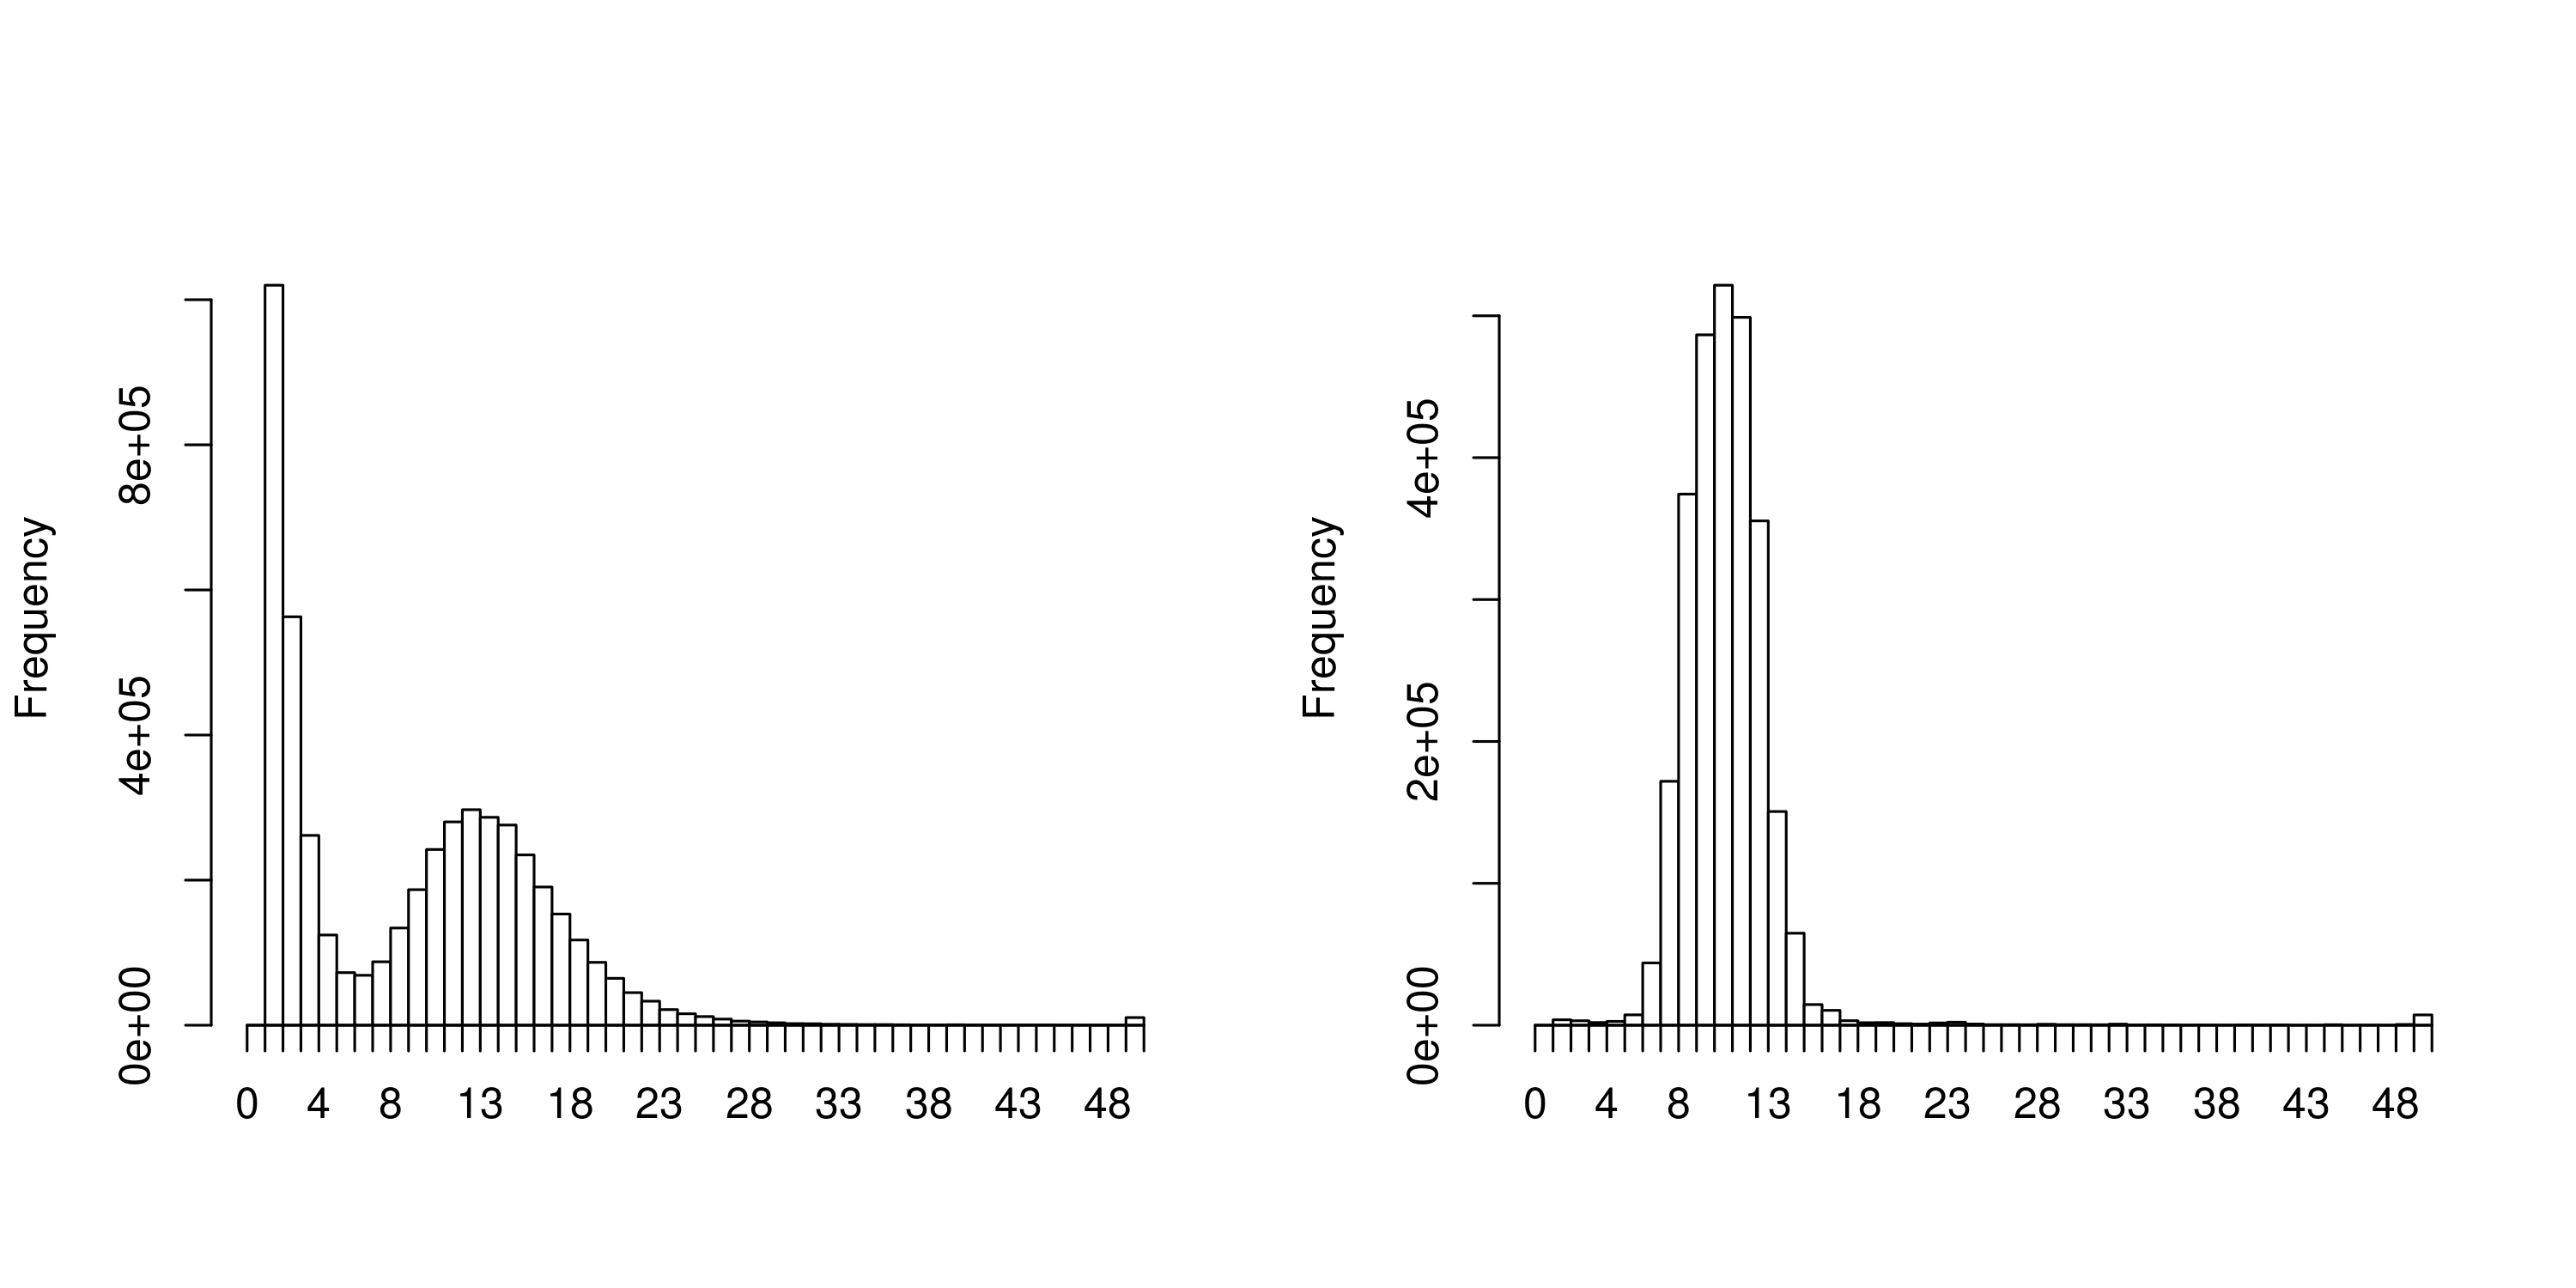
\includegraphics[width=0.8\textwidth]{de_novo/velvet_Rplot002.png}
\label{fig:velvet_Rplot002}
\end{figure}

For me the histogram suggests to me to choose a coverage cut-off of around 9
with an expected coverage of about 19. If you disagree, feel free to try
different settings, but first leave R before running \texttt{velvetg} with the
coverage parameters typing:
\begin{lstlisting}
q()

cp run_25/contigs.fa run_25/contigs.fa.0

time velvetg run_25 -long_cov_cutoff 9
cp run_25/contigs.fa run_25/contigs.fa.1

time velvetg run_25 -long_cov_cutoff 9 -exp_cov 19
cp run_25/contigs.fa run_25/contigs.fa.2

gnx -min 100 -nx 25,50,75 run_25/contigs.fa.*
\end{lstlisting}

\end{steps}

\begin{questions}
What is the N50 and runtime using:
\texttt{-long\_cov\_cutoff 9}
  
\texttt{-long\_cov\_cutoff 9 -exp\_cov 19}
  
other runs?
    
Which other parameters could improve the assembly quality for long reads?

What do you think about assembling 454 reads with Velvet?
\end{questions}


\section{Assembling Mixed Insert Length Libraries}

\begin{note}
Like the previous examples, the data you will examine in this exercise is again
from Staphylococcus aureus which still has a genome of around 3MB. The reads are
Illumina paired end with an insert size of 170 bp and 350 bp.

You already downloaded the required reads from the SRA in previous exercises.
Specifically, the run data (SRR022863, SRR022852) from the SRA Study SRP001086.

\center{\url{http://www.ebi.ac.uk/ena/data/view/SRP001086}}
\end{note}

\begin{information}
The following exercise focuses on handing two insert length libraries with
velvet and the changes you have to look out for.
\end{information}

\begin{steps}
First move to the directory you made for this exercise, make a suitable named
directory for the exercise and check if all the files are in place:
\begin{lstlisting}
cd ~/NGS/velvet/part3
mkdir SRP001086
cd SRP001086
ln -s ~/NGS/Data/SRR022863_?.fastq.gz ./
ln -s ~/NGS/Data/SRR022852_?.fastq.gz ./
\end{lstlisting}

Now run \texttt{velveth} and \texttt{velvetg} using the appropriate command line
options by typing:
\begin{lstlisting}
time velveth run_25 25 -fmtAuto -create_binary -shortPaired -separate SRR022863_1.fastq.gz SRR022863_1.fastq.gz -shortPaired2 -separate SRR022852_1.fastq.gz SRR022852_2.fastq.gz
time velvetg run_25
\end{lstlisting}

The right thing to do is to run velvetg setting the cut-offs. To investigate
with R, as you did in the previous exercises, start up R and produce the
weighted histogram using the columns \texttt{short1\_cov} and
\texttt{short2\_cov} by typing:
\begin{lstlisting}
R --no-save
library(plotrix) 
data <- read.table("run_25/stats.txt", header=TRUE) 
weighted.hist(data$short1_cov+data$short2_cov, data$lgth, breaks=0:70)
\end{lstlisting}

\begin{figure}[H]
\centering
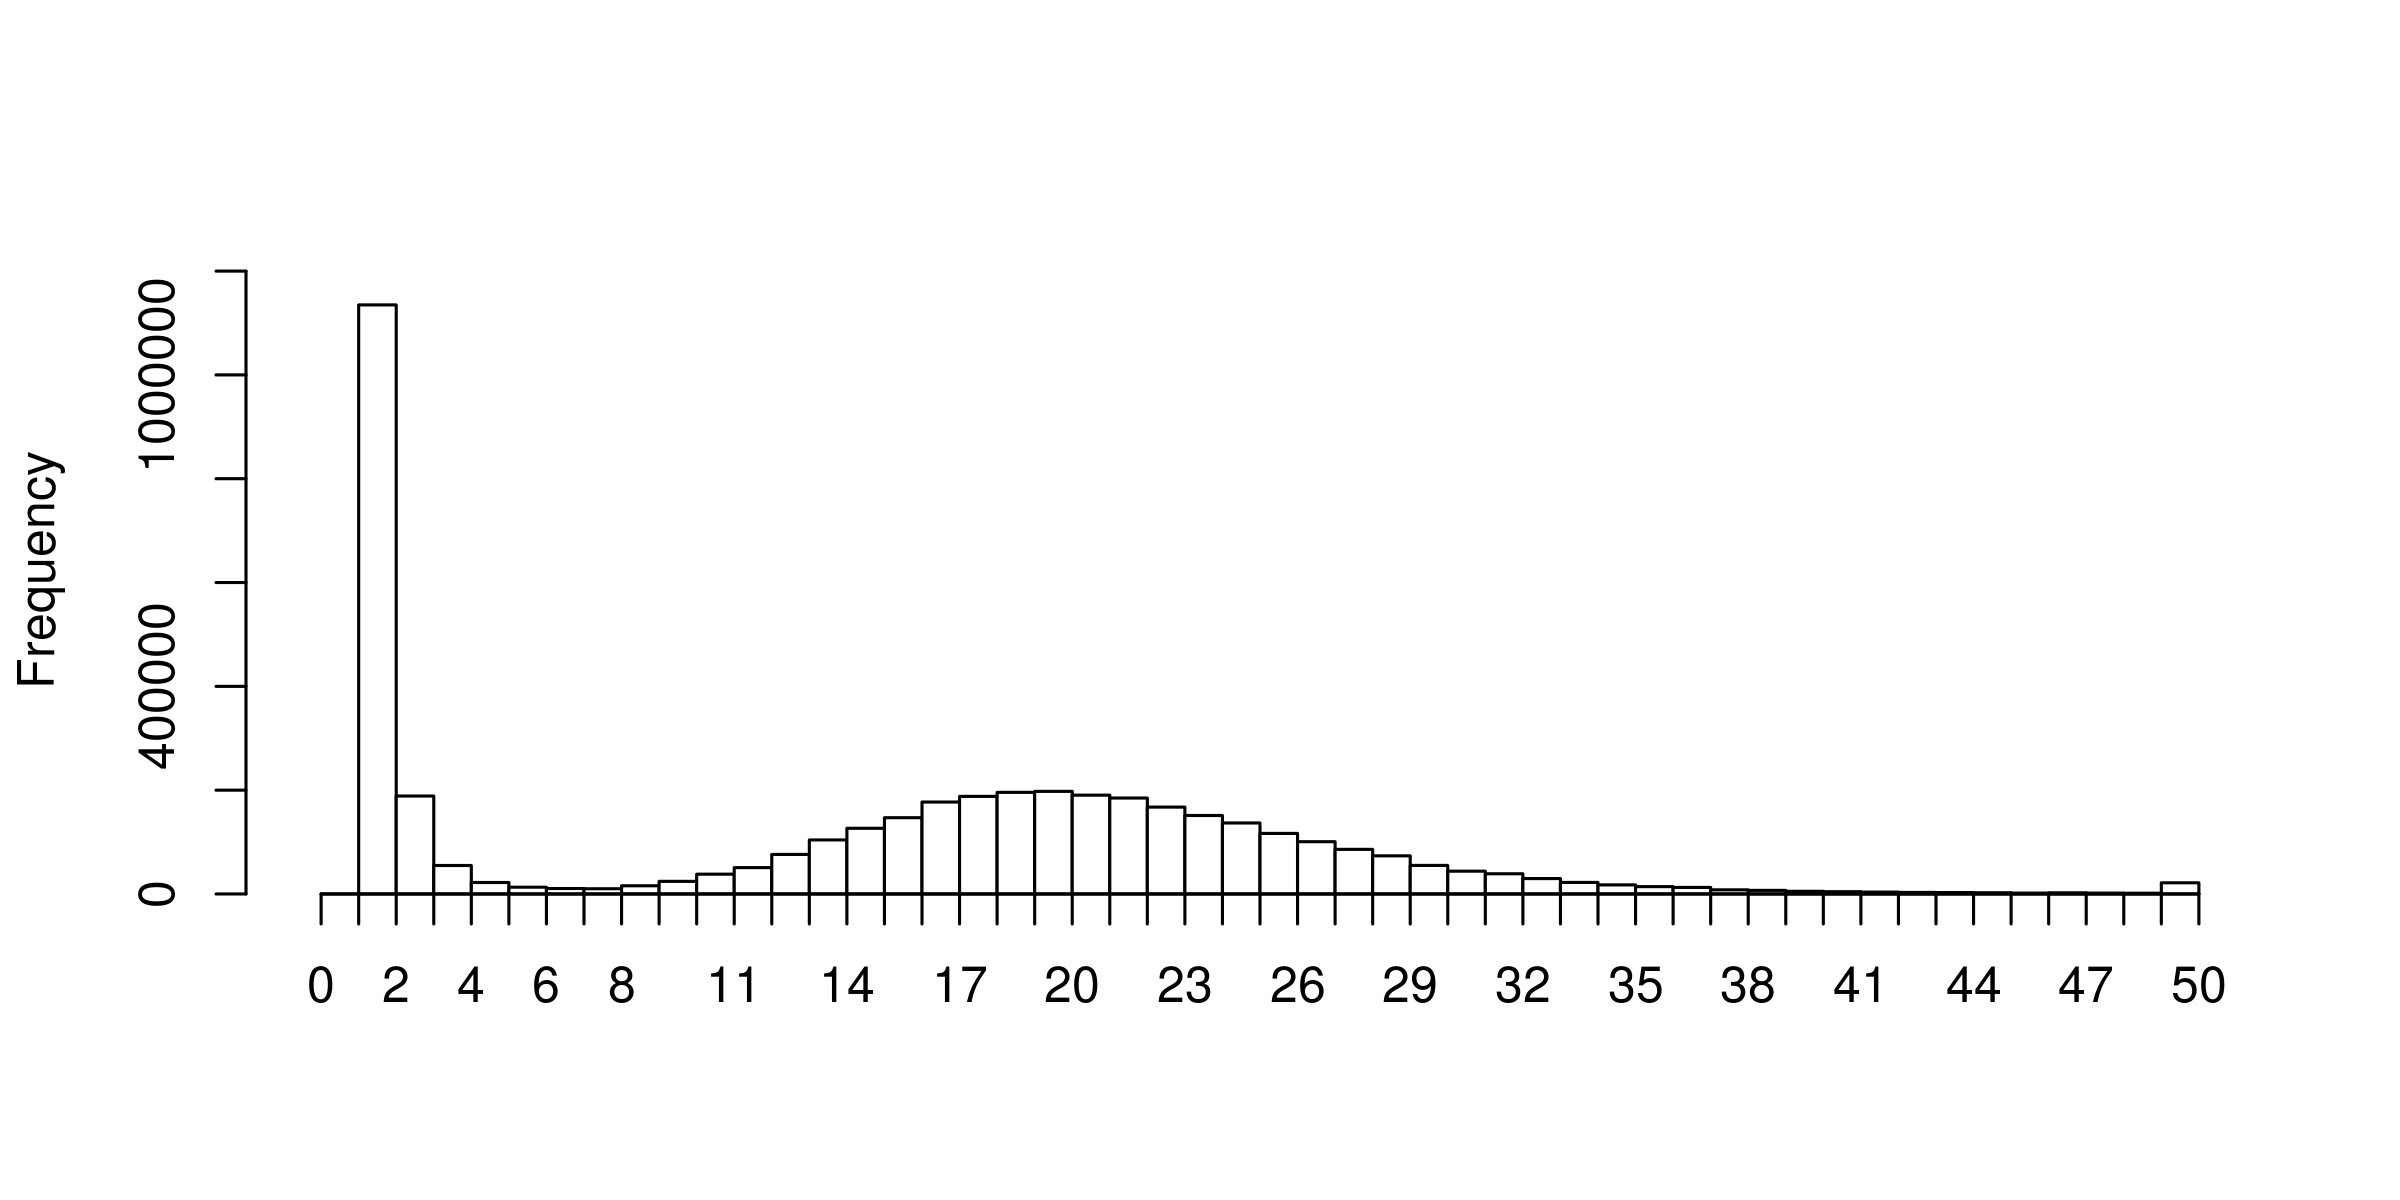
\includegraphics[width=0.8\textwidth]{de_novo/velvet_Rplot003.png}
\label{fig:velvet_Rplot003}
\end{figure}

For me the histogram suggests to me to choose a coverage cut-off of around 20
with an expected coverage of about 36. If you disagree, feel free to try
different settings, but first leave R before running velvetg with the coverage
parameters typing:
\begin{lstlisting}
q()

cp run_25/contigs.fa run_25/contigs.fa.0

time velvetg run_25 -cov_cutoff 20 
cp run_25/contigs.fa run_25/contigs.fa.1

time velvetg run_25 -cov_cutoff 20 -exp_cov 36 
cp run_25/contigs.fa run_25/contigs.fa.2

time velvetg run_25 -cov_cutoff 20 -exp_cov 36 -ins_length 170 -ins_length2 350
cp run_25/contigs.fa run_25/contigs.fa.3

gnx -min 100 -nx 25,50,75 run_25/contigs.fa.*
\end{lstlisting}

\end{steps}

\begin{questions}
What N50 did you get?

How did the runtime/results compare to one paired-end library runs?

How many different libraries would you be able to run with this velvet version?

Would you be able to add a single-end library as well with this velvet version?
\end{questions}

\begin{bonus}
Find and download a different insert length library
% TODO: \footnote affects the width of the shaded box - \renewcommand{\footnote}?
\footnotemark[1]
from the
study SRP001086 and recompile velvet to allow the use of three insert length
libraries. Maybe you could use the library you trimmed during previous
exercises. You should be able to find these files here:
\texttt{~/NGS/velvet/part2/SRX008042/SRR023408\_trim?.fastq}. If you don't still
have these files, you can find a copy of them here:
\texttt{~/NGS/Data/SRR023408\_trim?.fastq}.
Use the fresh compiled Velvet version with the three (two provided and one
downloaded library) to assemble the genome.
\begin{questions}
Does the extra library make any difference?
 
How does the overall coverage change?
 
Any other comments?
\end{questions}
\footnotetext[1]{Paired insert
lengths can be found on the NCBI SRA page in the library section (Nominal
length) e.g. \url{http://www.ncbi.nlm.nih.gov/sra?term=SRR022866}}
\end{bonus}

\begin{advanced}
\section{Hybrid Assembly}
\begin{note}
Like the previous examples, the data you will examine in this exercise is again
from Staphylococcus aureus which has a genome of around 3MB. The reads are 454
single end and Illumina paired end with an insert size of 170 bp.
You already downloaded the required reads from the SRA in previous exercises.
Specifically, the run data (SRR022863, SRR000892, SRR000893) from the SRA
experiments SRX007709 and SRX000181.
\end{note}

\begin{information}
The following exercise focuses on handing 454 long reads and paired-end reads
with velvet and the differences in setting parameters.
\end{information}

\begin{steps}
First move to the directory you made for this exercise, make a suitable named
directory for the exercise and check if all the three files are in place:
\begin{lstlisting}
cd ~/NGS/velvet/part3
mkdir SRR000892-SRR022863 
cd SRR000892-SRR022863
ln -s ~/NGS/Data/SRR00089[2-3].fastq.gz ./   
ln -s ~/NGS/Data/SRR022863_?.fastq.gz ./
\end{lstlisting}
\end{steps}

\begin{warning}
The following command will run for a LONG time. This indicated the amount of
calculations being preformed by Velvet to reach a conclusion. To wait for velvet
to finish would exceed the time available in this workshop, but it is up to you
to either let it run over night or kill the process by using the key combination
\texttt{CTRL+c}.
\begin{lstlisting}
velveth run_25 25 -fmtAuto -create_binary -long SRR00089?.fastq.gz -shortPaired -separate SRR022863_1.fastq.gz SRR022863_2.fastq.gz
time velvetg run_25
\end{lstlisting}

\begin{steps}
If you have decided to continue, we already inspected the weighted histograms
for the short and long read library separately, you can reuse this for the
cut-off values:
\begin{lstlisting}
time velvetg run_25 -cov_cutoff 7 -long_cov_cutoff 9
\end{lstlisting}
\end{steps}

\begin{questions}
What are your conclusions using velvet in an hybrid assembly?
\end{questions}

\end{warning}




\end{advanced}











\chapterstyle{workshop}